Hoy os voy a hablar de algo en lo que suele haber bastante lío en LaTeX:
la configuración de idioma. Creo que he conseguido más o menos entender
cómo va, así que voy a intentar explicar qué paquetes tenemos que usar y
por qué. Es una entrada que entra bastante en detalle, porque me gusta
saber el motivo de hacer las cosas, si no os apetece leer toda la chapa
(es mucha chapa) podéis ir directamente al resumen final.

Si no escribimos en inglés, tenemos que configurar LaTeX para que se
adapte a nuestro idioma. Para ello, necesitamos elegir un paquete de
idioma y una codificación.

\section{El paquete de idioma}\label{sec:paqueteIdioma}

El paquete de idioma realiza dos funciones principales:

\begin{itemize}
\item
  Gestiona que las palabras claves como Capítulo o la fecha se escriban
  en el idioma que hemos elegido.
\item
  Aplica la silabación\footnote{Por dónde nos parte una palabra cuando no cabe en
  la línea} correcta para el idioma concreto, así como otras reglas
  tipográficas.
\end{itemize}

Dependiendo de qué compilador estemos usando tendremos que usar un
paquete de idioma u otro:

\begin{itemize}
\item
  Si usamos \lstinline!pdflatex!, necesitamos cargar el paquete \lstinline!babel! con el idioma
  elegido como opción, por ejemplo:
\end{itemize}

\begin{lstlisting}[language={[latex]tex}]
\usepackage[spanish]{babel}
\end{lstlisting}

\begin{itemize}
\item
  Si usamos compiladores más modernos como \lstinline!xelatex! o \lstinline!lualatex!, podemos
  usar el paquete \lstinline!polyglossia!\footnote{Digo podemos porque, menos en algún caso
  especial, \texttt{babel} también funciona.}. Este paquete es más simple y
  ligero aprovechando que estos compiladores ya gestionan la
  codificación y las fuentes de por sí. En este caso no cargamos el
  idioma como opción, sino que lo elegimos con el comando
  \lstinline!\setmainlanguage!:
\end{itemize}

\begin{lstlisting}[language={[latex]tex}]
\usepackage{polyglossia}
\setmainlanguage{spanish}
\end{lstlisting}

\subsection{Redefinir palabras clave}\label{sec:palabrasClave}

Nos puede pasar que no nos guste la palabra que el paquete de idioma
utiliza para referirse a cierta parte del documento, por ejemplo,
utilizando la opción de español LaTeX llamará \emph{Cuadro} a las tablas. Si es
así, podemos redefinir el nombre del elemento. Es sencillo, tenemos que
usar \lstinline!\renewcommand! con la siguiente estructura:

\begin{lstlisting}[language={[latex]tex}]
\renewcommand{Comando a redefinir}{Nueva definición}
\end{lstlisting}

Aquí, por supuesto, hay diferencias si usamos \lstinline!babel! o \lstinline!polyglossia!.

\subsubsection{El caso babel}

Si usamos \lstinline!babel!, el comando que redefiniremos tendrá un nombre formado
por el nombre del idioma y el nombre de la palabra clave. Por ejemplo,
para cambiar Cuadro por Tabla en español haríamos:

\begin{lstlisting}[language={[latex]tex}]
\renewcommand{\spanishtablename}{Tabla}
\end{lstlisting}

Del mismo modo, si queremos modificar cómo llama LaTeX a las figuras en
francés, redefiniríamos el comando \lstinline!\frenchfigurename! y así con todos.

\begin{figure}[htbp]
\centering
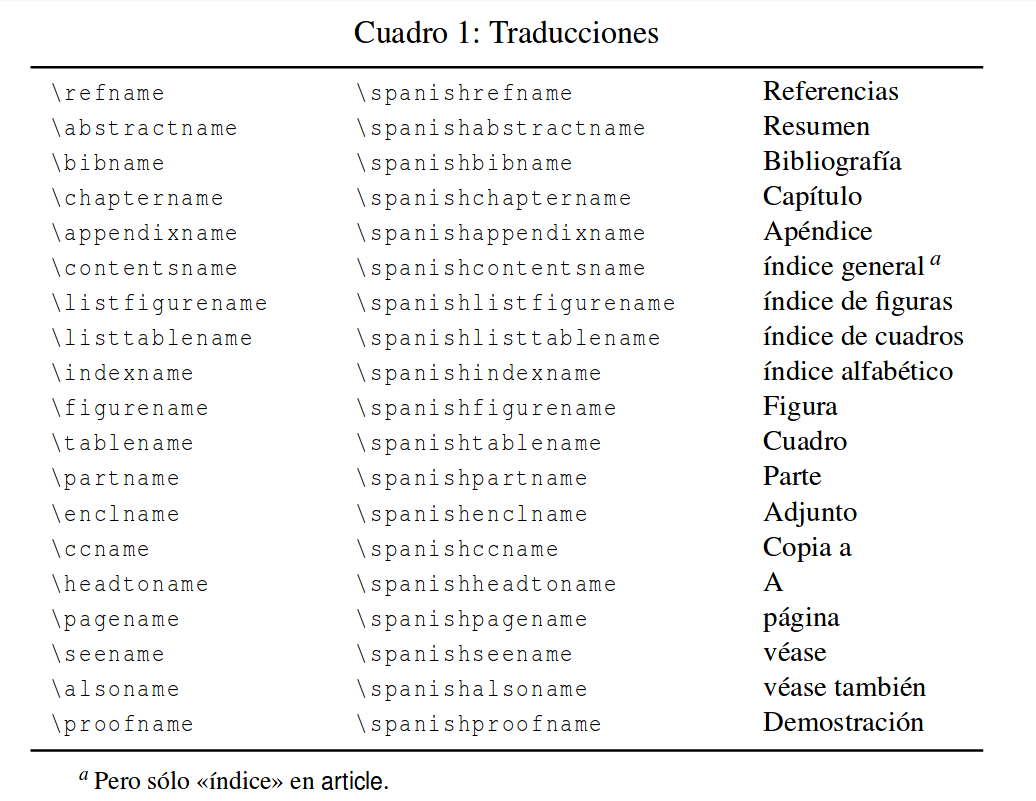
\includegraphics[width=0.9\textwidth]{docs/Figuras/traducciones}
\caption{Tabla que nos dice cómo llama a cada uno de los elementos. Del manual del estilo \lstinline!spanish! del paquete \lstinline!babel!}
\end{figure}

En el caso concreto de las tablas y para \lstinline!pdflatex! podemos cargar el
paquete \lstinline!babel! con la opción \lstinline!es-tabla! y nos evitamos problemas, pero para
el resto de elementos tenemos que hacer lo que os cuento.

\subsubsection{El caso polyglossia}

Si usamos \lstinline!polyglossia!, en su manual dicen que tenemos que cambiar el
nombre de la palabra clave con \lstinline!\gappto! (o \lstinline!\addto! para que sea compatible
con \lstinline!babel!)\footnote{A pesar de que \href{http://tex.stackexchange.com/questions/82993/how-to-change-the-name-of-document-elements-like-figure-contents-bibliogr}{leí} 
(y \href{https://ondahostil.wordpress.com/2017/02/09/lo-que-he-aprendido-establecer-el-idioma-para-xelatex/}{escribí}) que esos nombres se cambiaban
con el comando \texttt{\addto} en el manual de español de \lstinline!babel! dicen que es
mejor usar directamente renewcommand y spanishtablename o el nombre que corresponda.}. Por ejemplo:

\begin{lstlisting}[language={[latex]tex}]
\gappto\captionsspanish{\renewcommand{\tablename}{Tabla}}
\end{lstlisting}

\subsection{Texto en diferentes idiomas}\label{texto-en-diferentes-idiomas}

La última cosa que os voy a contar sobre los paquetes de idioma es cómo
cambiamos de idioma en un mismo documento.

\subsubsection{El caso \texttt{babel}}

En este caso simplemente cargamos como opciones del paquete \lstinline!babel! todos
los idiomas que vamos a usar en el documento:

\begin{lstlisting}[language={[latex]tex}]
\usepackage[idioma1, idioma2]{babel}
\end{lstlisting}

Los vamos activando en el texto con \lstinline!\selectlanguage!:

\begin{lstlisting}[language={[latex]tex}]
\usepackage[spanish, english]{babel}
\selectlanguage{spanish}

\begin{document}

  \section{Sección en español}

  \selectlanguage{english}
  \section{Section in english}

\end{document}
\end{lstlisting}

\subsubsection{El caso \texttt{polyglossia}}

Si estamos usando \lstinline!polyglossia!, cargamos el paquete y establecemos los
idiomas en el preámbulo de la siguiente manera:

\begin{lstlisting}[language={[latex]tex}]
\usepackage{polyglossia}
\setmainlanguage[Opciones]{Idioma} % Idioma principal
\setotherlanguage[Opcions]{Idioma} % Otro idioma
\end{lstlisting}

Si queremos cambiar el idioma de un trocito pequeño de texto usaremos el
comando \lstinline!\textIDIOMA!. Por ejemplo, para poner la fecha en español
haríamos:

\begin{lstlisting}[language={[latex]tex}]
\textspanish{\today}
\end{lstlisting}

Si vamos a escribir un pedazo de texto largo en otro idioma, es
preferible que usemos el entorno correspondiente al idioma;

\begin{lstlisting}[language={[latex]tex}]
\begin{spanish}
  Texto en español
\end{spanish}
\end{lstlisting}

\section{La codificación}\label{sec:codificacion}

La otra parte importante a la hora de configurar el idioma en LaTeX es
la codificación. Hay dos tipos de codificación: la codificación de
entrada y la codificación de fuente.

Configurar la codificación de entrada correctamente para nuestro idioma
nos permite escribir directamente los caracteres especiales desde el
teclado, por ejemplo, poder poner \lstinline!á! en lugar de \lstinline!\'a!.

Una codificación de fuente correcta, por su parte, sirve para que LaTeX
pueda partir las palabras por donde debe y para que podamos buscar en el
pdf resultante palabras con caracteres especiales. Si usamos una
codificación de fuente inadecuada ocurren cosas curiosas como que no
podamos copiar de un pdf palabras que contengan \emph{fi}. Esto se debe a que
LaTeX trata \emph{fi} como un único carácter, ya que es una \href{https://es.wikipedia.org/wiki/Ligadura_(tipograf\%C3\%ADa)}{ligadura
tipográfica}.

Aquí nos ocurre exactamente lo mismo que antes, dependiendo del
compilador tenemos que usar o no diferentes paquetes.

\subsection{El caso de pdflatex}\label{sec:pdflatex}

El pobre \lstinline!pdflatex! es viejecito y necesita ayuda para gestionar la
codificación. Nos hacen falta los siguientes paquetes:

\begin{itemize}
\item
  \lstinline!inputenc!: gestiona la codificación de entrada. Como opción le daremos
  la codificación, para ahorrarnos problemas usaremos \href{https://en.wikipedia.org/wiki/UTF-8}{UTF 8}
\item
  \lstinline!fontenc!: gestiona la codificación de fuente. Para escribir en
  castellano, usaremos la codificación \href{https://en.wikipedia.org/wiki/Cork_encoding}{T1} que contiene los caracteres
  necesarios de los idiomas que usan alfabeto latino con acentos. Si
  queréis escribir en cirílico no os vale esta codificación, tendréis
  que usar la T2A.
\item
  \lstinline!lmodern! o \lstinline!cm-super!: la fuente que LaTeX usa por defecto, Computer
  Modern, no es compatible con la codificación T1 así que necesitaremos
  usar su variante Latin Modern (paquete \lstinline!lmodern!) o la Computer Modern
  Super (paquete \lstinline!cm-super!). Parece ser que la Latin Modern es mejor para
  los acentos y la CM Super para el cirílico.
\end{itemize}

Si queremos escribir en español, la parte del idioma en el preámbulo
para \lstinline!pdflatex! nos queda por lo tanto así:

\begin{lstlisting}[language={[latex]tex}]
\usepackage[spanish]{babel}
\usepackage[utf8]{inputenc} 
\usepackage[T1]{fontenc}
\usepackage{lmodern}
\end{lstlisting}

Para cualquier otro idioma con acentos o caracteres especiales
necesitamos los mismos paquetes y solo tendríamos que cambiar la opción
de idioma en el paquete \lstinline!babel!.

\subsection{Xelatex y otros compiladores
modernos}\label{sec:xelatex}

Los compiladores modernos gestionan ellos solitos la codificación de
entrada y la de fuente así que no es necesario que añadamos ningún
paquete extra. Qué bien ¿eh?

\section{En resumen, ¿qué hago?}\label{sec:resumen6}

Después de todo el rollo que os he soltado, vamos a recapitular y ver
qué necesitamos en cada caso.

Para compilar con \lstinline!pdflatex! añadimos esto al preámbulo:

\begin{lstlisting}[language={[latex]tex}]
\usepackage[spanish,es-tabla]{babel} % Cargamos es-tabla para Tabla en lugar de Cuadro
\usepackage[utf8]{inputenc} % Codificación de entrada
\usepackage[T1]{fontenc} % Codificación de fuente
\usepackage{lmodern} % Fuente compatible
\end{lstlisting}

Para compilar con \lstinline!xelatex! añadimos esto al preámbulo:

\begin{lstlisting}[language={[latex]tex}]
\usepackage{polyglossia}
\setmainlanguage{spanish}
% Para Tabla en lugar de Cuadro
\gappto\captionsspanish{\renewcommand{\tablename}{Tabla}} 
\end{lstlisting}

Podemos venirnos arriba, utilizar el paquete \lstinline!ifxetex! (que mira si
estamos compilando con \lstinline!xelatex!), añadir este trocito al preámbulo y
asegurar que funciona con los dos compiladores:

\begin{lstlisting}[language={[latex]tex}]
% Idioma
\ifxetex
  \usepackage{polyglossia}
  \setmainlanguage{spanish}

  % Tabla en lugar de cuadro
  \gappto\captionsspanish{\renewcommand{\tablename}{Tabla}  
          \renewcommand{\listtablename}{Índice de tablas}}

\else
  \usepackage[spanish,es-tabla]{babel}
  % Para los acentos (xelatex no lo necesita)
  \usepackage[utf8]{inputenc} 
  \usepackage[T1]{fontenc}
  \usepackage{lmodern}
\fi
\end{lstlisting}

Os he añadido la parte de cambiar \emph{Cuadro} por \emph{Tabla} pero, por supuesto,
no es necesario.

\section{Referencias}

\href{http://osl.ugr.es/CTAN/macros/latex/required/babel/base/babel.pdf}{Manual
del paquete \texttt{babel} (pdf)}

\href{http://tug.ctan.org/tex-archive/language/spanish/babel/base/spanish.pdf}{\emph{Estilo
spanish para el sistema babel} (pdf)}

\href{http://osl.ugr.es/CTAN/macros/latex/contrib/polyglossia/polyglossia.pdf}{Manual
del paquete \texttt{polyglossia} (pdf)}

\href{http://mirror.utexas.edu/ctan/macros/latex/doc/encguide.pdf}{\emph{LaTeX
font encodings}}
